
\documentclass[11pt]{article}
\usepackage[margin=1in]{geometry}
\usepackage{caption} %For captioning objects
\usepackage{subcaption} %sub-captioning pictures
\usepackage{graphicx} %to include graphics
\usepackage{hyperref} %for clickable references
\usepackage{listings} %to write code listings
\lstset{language=R, breaklines=true}  
\usepackage[mathcal]{euscript} %for curly S
\usepackage{mathtools}
\usepackage{float} %so figures can be placed "here"

%Defining commands for math symbols
\usepackage{amsmath} %to enable split equations
\usepackage{statmath} %for plim. Be careful, it has already \E and \V.
\usepackage{amssymb} %to enable mathbb
\newcommand{\R}{\mathtt{R}} %Software R
\renewcommand{\E}{\mathbb{E}} %expectation
\usepackage{bbm}
\newcommand{\1}{\mathbbm{1}}
\renewcommand{\V}{\mathbb{V}} %variance
\newcommand{\N}{\mathcal{N}} %normal distribution
\newcommand{\U}{\mathcal{U}} %normal distribution
\renewcommand{\P}{\mathbb{P}} %proba, renewcom since \P already exists
%Regression variables in vector form
\newcommand{\y}{\boldsymbol{y}} 
\newcommand{\x}{\boldsymbol{x}} 
\newcommand{\z}{\boldsymbol{z}} 
\newcommand{\yhat}{\boldsymbol{\hat{y}}} 
\renewcommand{\u}{\boldsymbol{u}} 
\newcommand{\uhat}{\boldsymbol{\hat{u}}}  
\newcommand{\Px}{\boldsymbol{P}}  
\newcommand{\Mx}{\boldsymbol{M}}  
\newcommand{\A}{\boldsymbol{A}}  
\newcommand{\X}{\boldsymbol{X}}  
\newcommand{\Z}{\boldsymbol{Z}}  
\newcommand{\e}{\boldsymbol{e}}  
\renewcommand{\r}{\tilde{r}}  
%\renewcommand{\r}{\boldsymbol{r}} 
\renewcommand{\i}{\boldsymbol{\imath}} 
\newcommand{\alphab}{\boldsymbol{\alpha}}  
\newcommand{\betab}{\boldsymbol{\beta}}  
%opening

\newcounter{daggerfootnote}
\newcommand*{\daggerfootnote}[1]{%
	\setcounter{daggerfootnote}{\value{footnote}}%
	\renewcommand*{\thefootnote}{\fnsymbol{footnote}}%
	\footnote[2]{#1}%
	\setcounter{footnote}{\value{daggerfootnote}}%
	\renewcommand*{\thefootnote}{\arabic{footnote}}%
}


\title{Problem Set 5 - ECON 880\\
	\small Spring 2022 - University of Kansas}
\author{Gunawan, Minh Cao}


\begin{document}

\maketitle	
\section*{Question 1}
We have given $f(x) = (x^{1/2}+1)^{2/3}$, with a starting value $x_0=1$. The first derivative is given by
\[ f'(x) = \frac{1}{3x^{1/2}(x^{1/2} + 1)^{1/3}},\]
while the second one is given by
\[f''(x)= \frac{-1}{18x(x^{1/2} + 1)^{4/3}} - \frac{1}{6x^{3/2}(x^{1/2} + 1)^{1/3}}\]

\subsection*{1(a) Taylor Series Approximation }
The first-order Taylor series approximation is given by:
\begin{eqnarray*}
	f(x) &=& f(x_0)+f'(x_0)(x-x_0)\\
		 &=& 1.5874 + 0.2646 (x-1)
\end{eqnarray*}
The second-order Taylor series approximation is given by:
\begin{eqnarray*}
	f(x) &=& f(x_0)+f'(x_0)(x-x_0)+\frac{(x-x_0)^2}{2}f''(x_0)\\
	&=& 1.5874 + 0.2646 (x-1) -0.0772 (x-1)^2
\end{eqnarray*}
\subsection*{1(b) Pad\'{e} Approximation}
We want to compute Pad\'{e} Approximation (1,1) 
\[P_{M=1}^{N=1}(x) = \frac{a_0+a_1(x-x_0)}{b_0+b_1(x-x_0)},\]
where $b_0=1$ (normalized). 
The Pad\'{e} coefficients are normally best found from an $(M+N)$\textsuperscript{-th} order Taylor series expansion of $f(x)$ :
\begin{eqnarray*}
	T_2(x) &=& \frac{a_0+a_1(x-1)}{1+b_1(x-1)}\\
	1.5874 + 0.2646 (x-1) -0.0772 (x-1)^2 &=&  \frac{a_0+a_1(x-1)}{1+b_1(x-1)}
\end{eqnarray*}
Multiplying up the denominator of the RHS with the LHS gives the following equivalent set of coefficient relations:
\begin{eqnarray}
	a_0 &=& 1.5874 \label{1b:1}\\
	a_1 &=&  1.5874b_1 + 0.2646 \label{1b:2}\\
	0	&=& 0.2646b_1 -0.0772 \label{1b:3} 
\end{eqnarray}
From equation \ref{1b:3}, we obtain $b_1=0.2917$. Then, we plug it in into equation \ref{1b:2} to obtain $a_1=0.7276$. Finally, the Pad\'{e} Approximation (1,1) for $f(x)$ is given by
\[P_{M=1}^{N=1}(x) = \frac{1.5874+0.7276(x-1)}{1+0.2917(x-1)},\]
\section*{Question 2}
Consider the function 
\[f (x ) = e^{4x-2} \]
over $[0,2]$ interval, and construct the following approximations
to it:
\begin{enumerate}
	\item[(a)] Chebyshev polynomials of degree 4; choose 5 points to use as nodes.
	\item[(b)] Cubic spline over 5 equally spaced points in $[0,2]$.
\end{enumerate}
Then evaluate the approximations over 101 equally spaced points in $[0,2]$ and plot them along with the true function. 

\subsection*{2(a) Chebyshev Interpolation}
We use the following algorithm\daggerfootnote{Kenneth L. Judd, 1998. "Numerical Methods in Economics," MIT Press Books, The MIT Press, p.223} to construct the Chebyshev interpolation of order 4. The result is shown on Figure \ref{2a:1}.
\begin{enumerate}
	\item [Step 1.] Compute five Chebyshev interpolation nodes on $[0,2]$ using the following formula
	\[z_k = -\cos\left(\frac{2k-1}{2m}\pi\right), \quad k=1,\ldots,m\]
	\item[Step 2.] Adjust the nodes to the $[0,2]$ interval:
	\[x_k=(z_k+1)\left(\frac{2-0}{2}\right)+0=z_k+1,\quad k=1,\ldots,m\]
	\item[Step 3.] Evaluate $f$ at the approximation nodes
	\[y_k=f(x_k), \quad k=1,\ldots,m\]
	\item[Step 4.] Compute Chebyshev coefficients $\{a_i\}_{i=0}^n$
	\[a_i=\frac{\sum_{k=1}^my_kT_i(z_k)}{\sum_{k=1}^mT_i(z_k)^2},\]
	where $T_i(x)=2xT_{i-1}(x)-T_{i-2}(x)$, with $T_0(x)=1$ and $T_1(x)=x$, for $i=2,\ldots,n$
	\item[Step 5.] The approximation for $f(x)$, $x\in[0,2]$ is given by:
	\[\hat{f}(x)=\sum_{i=0}^n a_iT_i\left(x-1\right).\]
\end{enumerate}


\subsection*{2(a) Cubic Spline Interpolation}
We use the following algorithm to construct the cubic spline interpolation. The result is shown on Figure \ref{2a:1}.
\begin{enumerate}
	\item [Step 1.] xxx
	\item[Step 2.] xxx
	\item[Step 3.] xxx
	\item[Step 4.] xxx
	\item[Step 5.] xxx
\end{enumerate}

Comment: which method works better? Are higher order Chebyshev coefficients indeed smaller? Do approximations match the slope and curvature of the original function?

\begin{figure}[h]
	\centering
		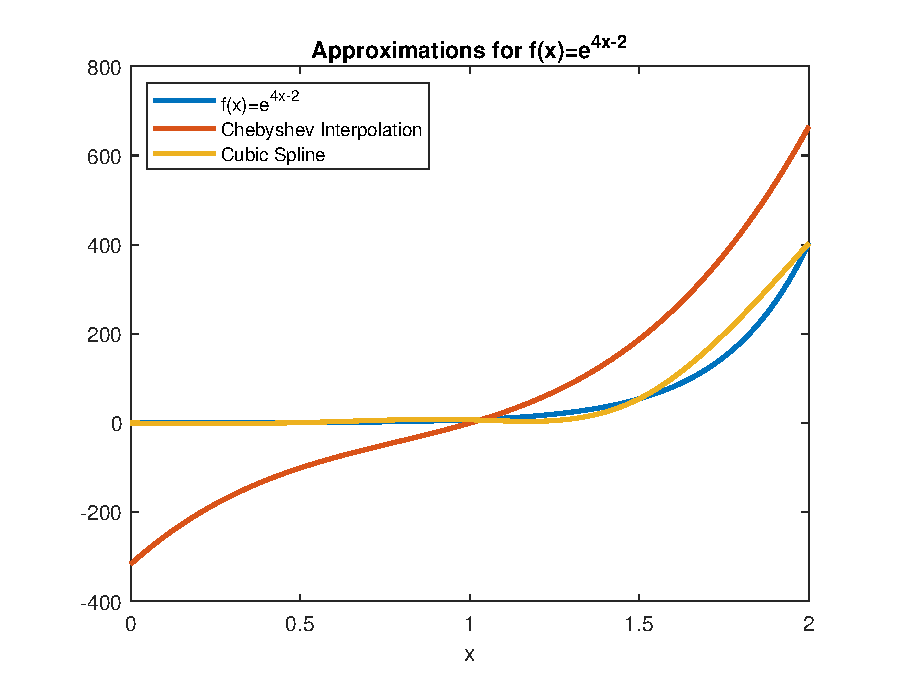
\includegraphics[width=\textwidth]{fig1.eps}
	\caption{Approximations for $f(x)=e^{4x-2}$}
	\label{2a:1}
\end{figure}

\end{document}

